\documentclass[12pt,a4paper]{article}
\usepackage{polski}
\usepackage[utf8]{inputenc}
\usepackage{amsmath}
\usepackage{amssymb}
\usepackage{amsfonts}
\usepackage{graphicx}
\usepackage{placeins}
\usepackage{listings}
\usepackage[svgnames]{xcolor}
 \lstset{literate={ą}{{\k{a}}}1 {ć}{{\'c}}1 {ę}{{\k{e}}}1 {ł}{{\l{}}}1 {ń}{{\'n}}1 {ó}{{\'o}}1 {ś}{{\'s}}1 {ż}{{\.z}}1 {ź}{{\'z}}1 {Ą}{{\k{A}}}1 {Ć}{{\'C}}1 {Ę}{{\k{E}}}1 {Ł}{{\L{}}}1 {Ń}{{\'N}}1 {Ó}{{\'O}}1 {Ś}{{\'S}}1 {Ż}{{\.Z}}1 {Ź}{{\'Z}}1 }
 \lstset{breaklines=true}
\lstset{language=Matlab,
  keywords={break,case,catch,continue,else,elseif,end,for,function,
     global,if,otherwise,persistent,return,switch,try,while},
  basicstyle=\ttfamily,
  keywordstyle=\color{blue},
  commentstyle=\color{DarkGreen},
  stringstyle=\color{dkgreen},
  numbers=left,
  numberstyle=\tiny\color{gray},
  stepnumber=1,
  numbersep=10pt,
  backgroundcolor=\color{white},
  tabsize=4,
  showspaces=false,
  showstringspaces=false}
  
\begin {document}
\begin{center}
\begin{large}
ATR --Average True Rang-  opis wskaźnika  \\
\end{large}
Łukasz Brzosko
\end{center}
%\baselineskip=22pt

Average True Range - średni zakres zmian. Jest to wskaźnik obliczający zmienność cen w ujęciu bezwględnym.  Wykorzystywany jest do wychwycenia zmienności kursu. Wskaźnik ATR oblicza się jako średnią z rzeczywistego zakresu zmian (TR - True Range), który jest największą wartością z następujących trzech wielkości : odległością pomiędzy poprzednią ceną zamknięcia (Close) a dzisiejszym minimum (Low),odległością pomiędzy dzisiejszym maksimum (High) a poprzednią ceną zamknięcia (Close),odległością pomiędzy dzisiejszym maksimum (High) i minimum (Low). Wskaźnik jest używany do przewidywania lokalnych szczytów i dołków - jego wartość jest często wysoka i osiąga szczyt przed lokalnym minimum lub maksimum kursu . Także wysoka wartość wskaźnika podczas gwałtownego spadku lub wzrostu może zapowiadać dłuższą zmianę trendu. Niskie wartości wskaźnika potwierdzają trend horyzontalny.



\noindent

\noindent Poniższy listing przedstawia zaimplementowaną strategię w MATLAB-ie.
\begin{scriptsize}
\begin{lstlisting}


%Dane:
tStart=tic;
cSizes = size(C);
candlesCount = cSizes(1);
kon=candlesCount-1;
sumRa=zeros(1,candlesCount);
Ra=zeros(1,candlesCount);
pocz=50;
la=0; %liczba otwieranych pozycji
lastCandle = kon-16;
recordReturn=0; %rekord zysku
recordDrawdown=0; %rekord obsuniecia
pic1 = false;
obv=C(pocz-1,5)
for i=pocz:lastCandle
 
   
    
    
       if(C(i,4)>C(i-1,4))
       obv_tab(i)=obv+C(i,5);
       obv=obv_tab(i);
       end
       if(C(i,4)<C(i-1,4))
       obv_tab(i)=obv-C(i,5);
       obv=obv_tab(i);
       end
       
        
end

for i=100:lastCandle
obv_max(i)=max([obv_tab(i-14) obv_tab(i-13) obv_tab(i-12) obv_tab(i-11) obv_tab(i-10) obv_tab(i-9) obv_tab(i-8) obv_tab(i-7) obv_tab(i-6) obv_tab(i-5) obv_tab(i-4) obv_tab(i-3) obv_tab(i-2) obv_tab(i-1)]);
end

for i=100:lastCandle
    
    
            if (obv_tab(i)>obv_max(i))
            Ra(i)=C(i+1,4)-C(i+1,1)-spread; %zysk z i-tej pozycji long zamykanej na zamknieciu po paramADuration kroku
            
            la=la+1;
      
            end
    sumRa(i)=sumRa(i-1) + Ra(i); %krzywa narastania kapita3u
    
    if sumRa(i)>recordReturn
        recordReturn=sumRa(i);
    end
    
    if sumRa(i)-recordReturn<recordDrawdown
        recordDrawdown=sumRa(i)-recordReturn; %obsuniecie maksymalne
    end
end

sumReturn=sumRa(lastCandle);




\end{lstlisting}
\end{scriptsize}


Na podstawie zebranych informacji dotyczących wskaźnika $ATR$ utworzono prostą strategię inwestycyjną bazującą na regule: Obliczono średnią ATR z 14 okresów i porównywano ją z wartością bezwględną z różnicy pomiędzy ceną otwarcia z aktualnej świecy, a ceną zaknięcia z poprzedzającej ceny. Jeżeli średnia była większa od wartości bezwględnej to zawierano transakcję kupna. Badania zostały przeprowadzone na parze walutowej $EURCZK$ (szereg czasowy przedstawiony na rysunku \ref{rysunek2}). \\
\begin{figure}[h!]
\centering
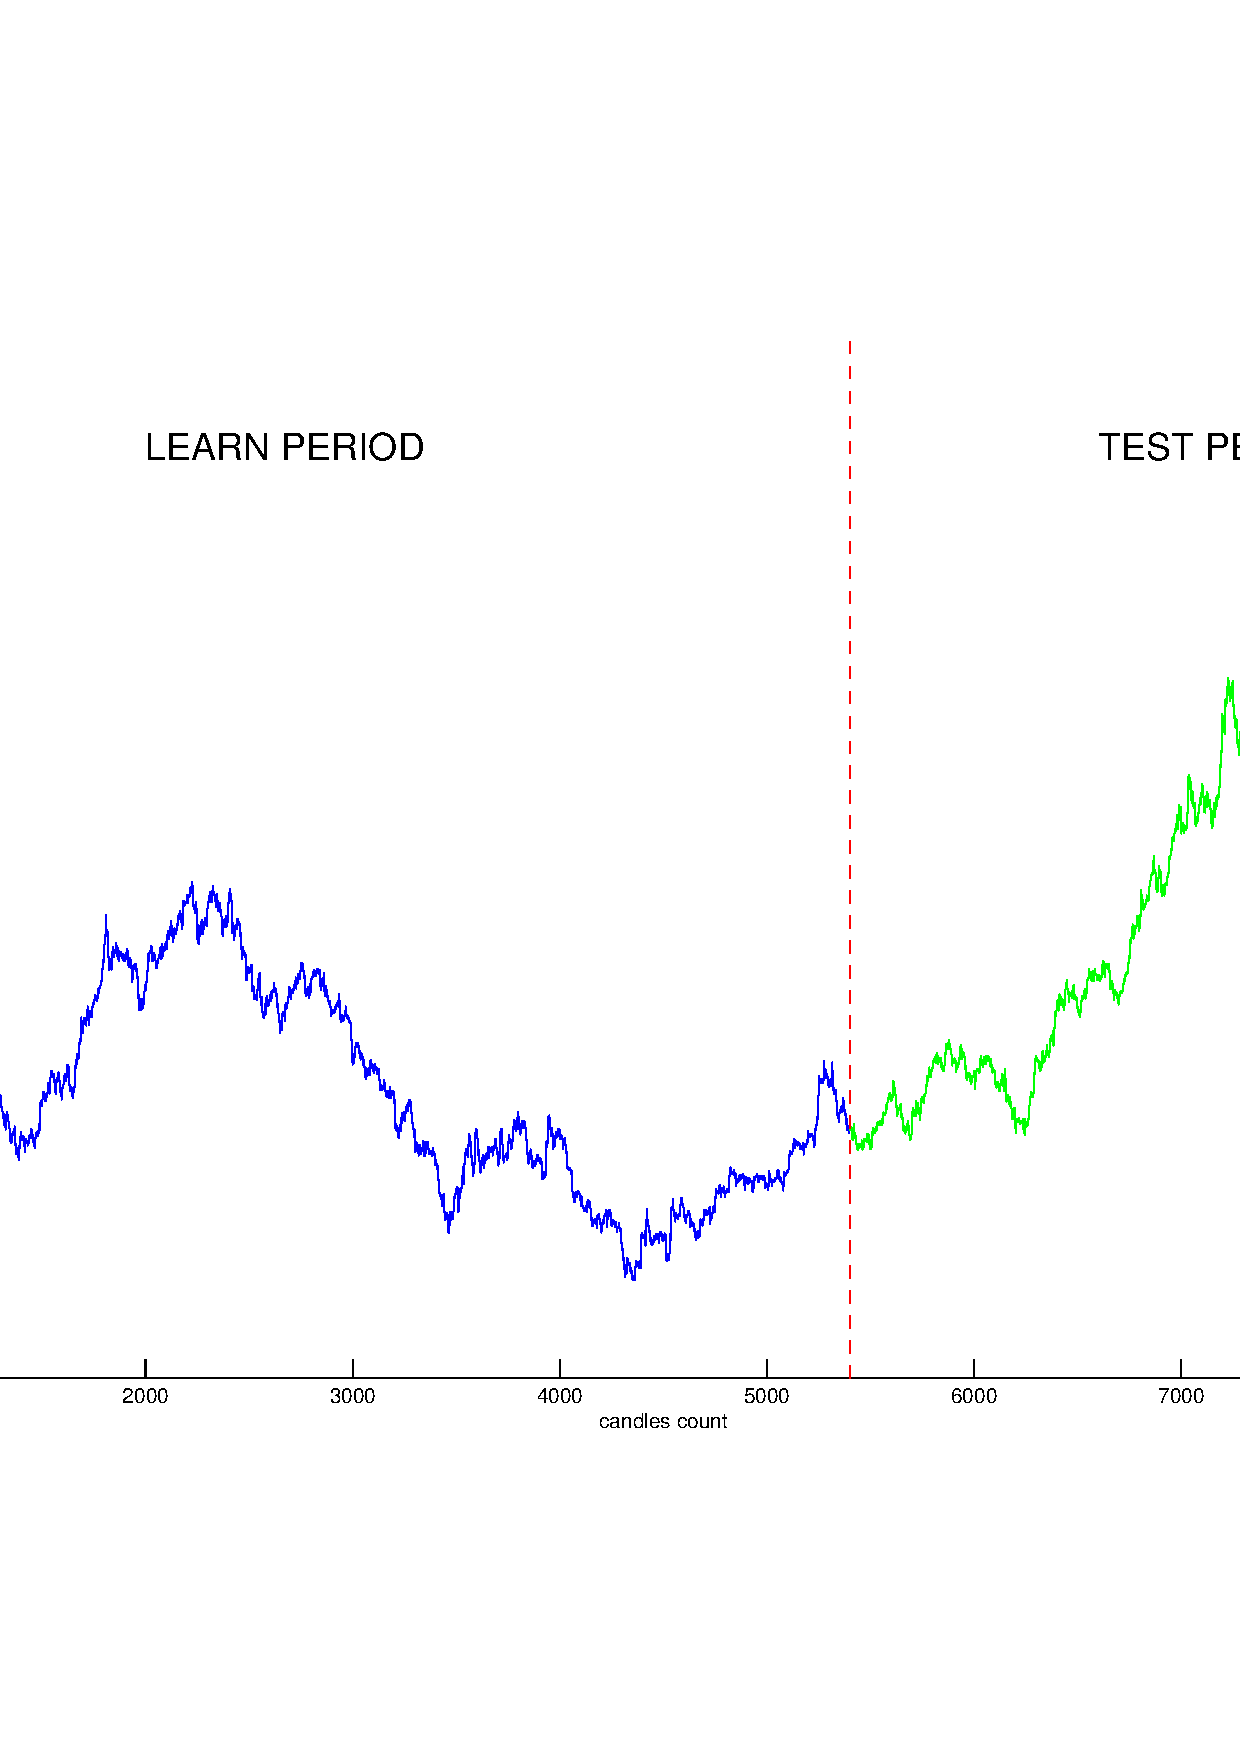
\includegraphics[width = \textwidth]{podzialDanych.png}
\caption{Badany szereg czasowy}
\label{rysunek2}
\end{figure}
\FloatBarrier
W przeprowadzonych badaniach przyjęto optymalną wartość parametru okresów do obliczenia wskaźnika ATR =14, następnie weryfikowano otrzymane wyniki na okresie testowym. 
\newpage
\noindent \textbf{I Wyniki badań .}\\
\begin{figure}[h!]
\centering
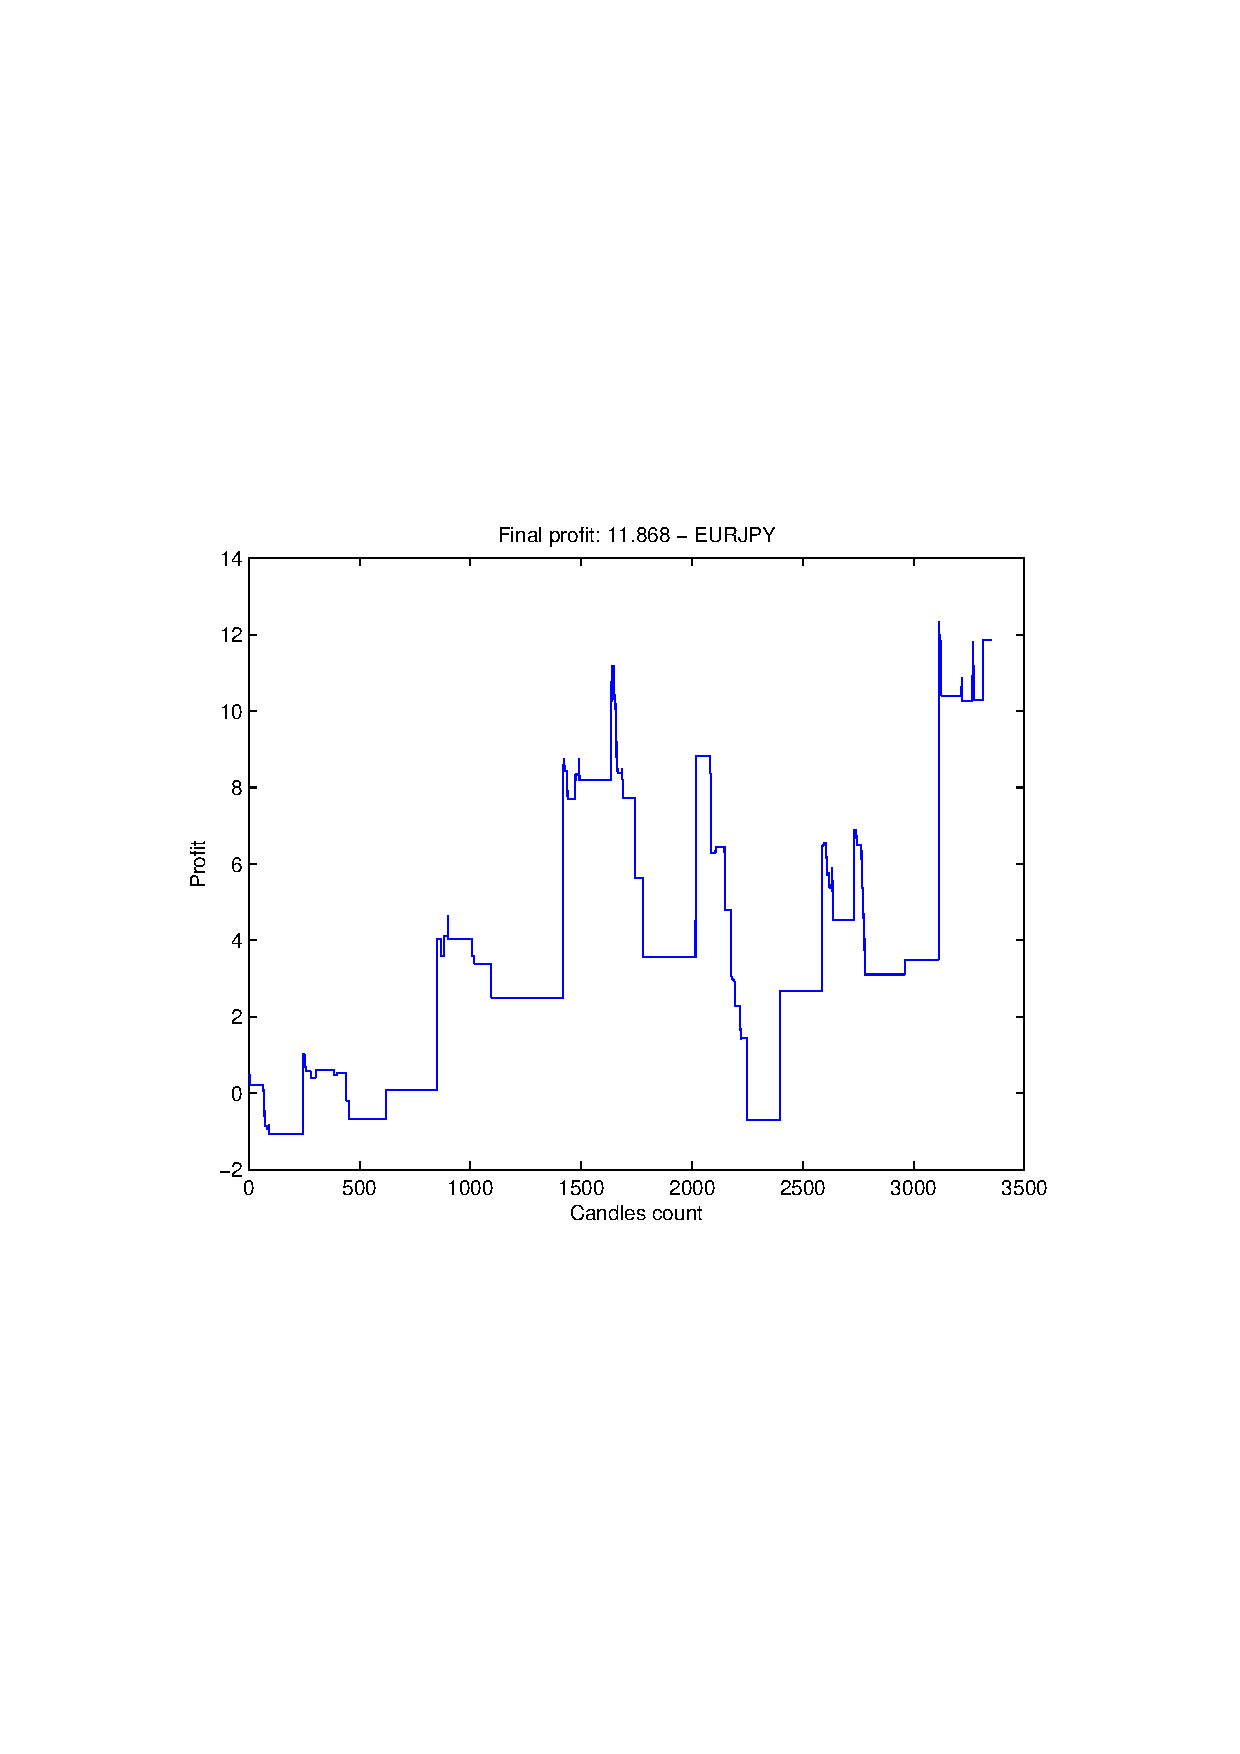
\includegraphics[width = 0.6\textwidth]{ROC_EURJPY_LS_SearchBestK_zysk.png}
\caption{Zysk skumulowany EURCZK na okresie testowym dla pozycji długich. }
\end{figure}
\FloatBarrier
\begin{verbatim}

Zysk skumulowany          18.4184
Calmar                     2.3641
liczba otwartych pozycji  8777





\end{verbatim}

\end {document}
